\section{Optimization}

\subsection{Linear Least Squares}

Suppose you had a set of noisy data that you would like to apply a curve fit to.

\begin{figure}[htb]
    \centering
    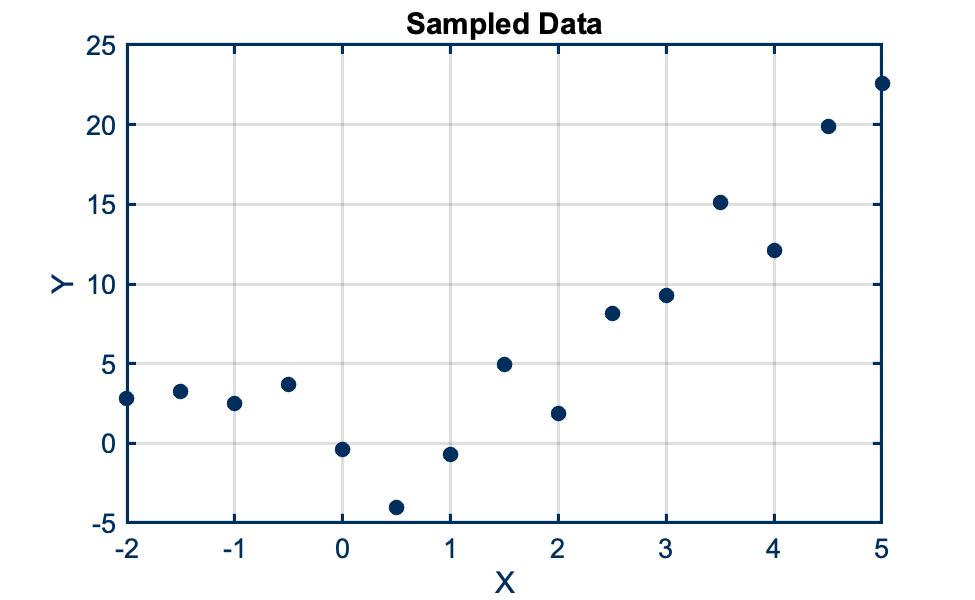
\includegraphics[width = 4 in]{Chapters/Computational Methods/Figures/Sample Linear Least Squares Data.png}
    \caption{Sample Linear Least Squares Data.}
    \label{fig:Sample Linear Least Squares Data}
\end{figure}

It just so happens that this

\subsubsection{Theory}

\begin{equation}
    \text{min} \sum_i \left[ \hat{f}\left(x^{(i)}\right) - f\left(x^{(i)} \right) \right]^2
\end{equation}